\section{Instrumental}
\subsection{Electrómetro Keithley 617}
Un electrómetro es un instrumento muy sensible para mediciones eléctricas.
Configurado para medir tensión, sus características son:
\begin{itemize}
    \item Alta impedancia de entrada:
\SI{200}{\tera\ohm} en paralelo con $<$\SI{2}{\pico\farad}
\item Alta precisión: $\pm0.05\%$
\item Alta resolución: hasta \SI{10}{\micro\volt}
\end{itemize}
\begin{figure}[p]
    \begin{subfigure}[b]{\textwidth}
    \centering
        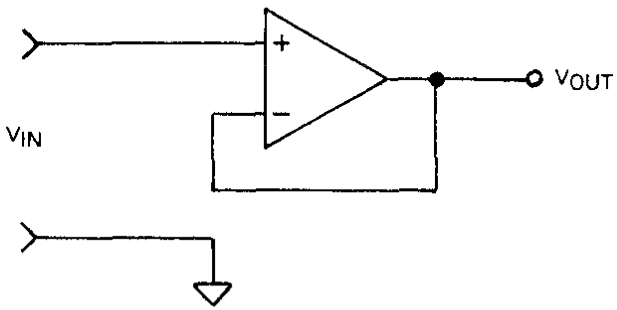
\includegraphics{figuras/instrumental/617volts.png}
        \caption{Tensión}
        %\label{fig:posicionno}
    \end{subfigure}
    \begin{subfigure}[b]{\textwidth}
    \centering
        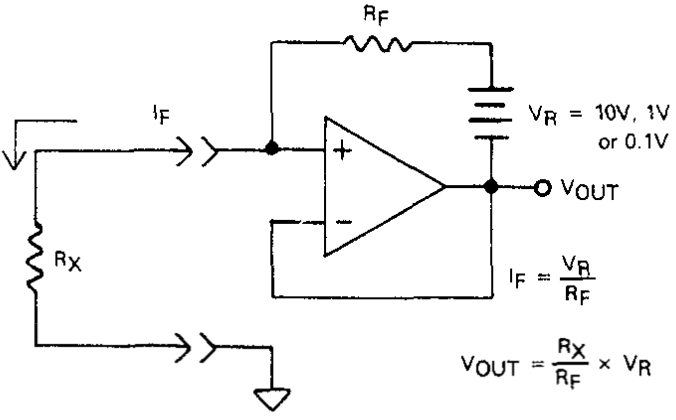
\includegraphics{figuras/instrumental/617ohms.png}
        \caption{Resistencia}
        %\label{fig:posicionno}
    \end{subfigure}
    \begin{subfigure}[b]{\textwidth}
    \centering
        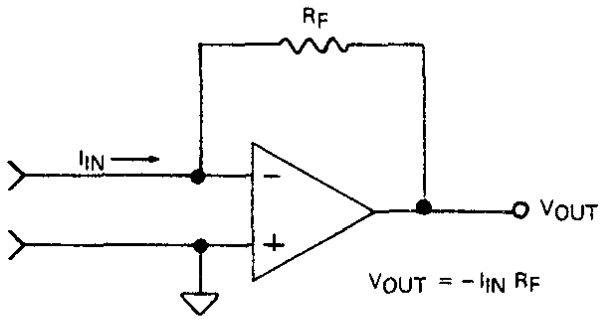
\includegraphics{figuras/instrumental/617amps.png}
        \caption{Corriente}
        %\label{fig:posicionno}
    \end{subfigure}
    \begin{subfigure}[b]{\textwidth}
    \centering
        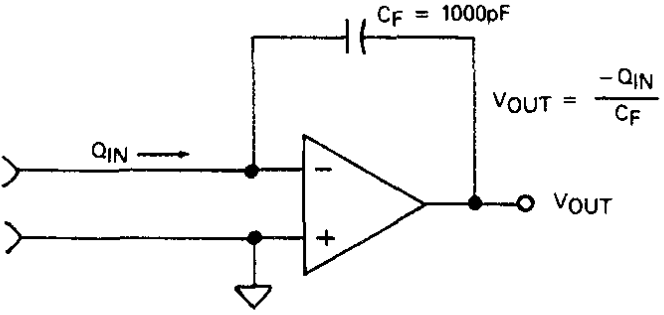
\includegraphics{figuras/instrumental/617coulombs.png}
        \caption{Carga}
        %\label{fig:posicionno}
    \end{subfigure}
    \caption{Configuraciones de medición del electrómetro.
    Reproducido de~\cite{keithley_instruments_inc._keithley_1984}.}
    \label{fig:keithley617}
\end{figure}
Introduciendo elementos de realimentación en el circuito de entrada,
es capaz de medir corriente, resistencia, carga y tensión
(\figref{fig:keithley617}).
La alta ganancia del amplificador mantiene la terminal de entrada a
\SI{0}{\volt}, 
evitando cargar el circuito bajo prueba.
La terminal de entrada está cuidadosamente aislada 
para evitar fugas de corriente. 
Por ejemplo, partes del circuito de entrada 
están levantadas del circuito impreso con aisladores de teflon
para aumentar la aislación.
\subsubsection{Medición con guarda}
Al medir una fuente de tensión de muy alta impedancia,
cualquier flujo de corriente hacia el instrumento de medición
provoca una caída de tensión considerable.
Debido a la alta impedancia de entrada del electrómetro,
fluye muy poca corriente a través de sus terminales.
Sin embargo, hay otra corriente que fluye en los cables debido a la resistencia
finita de la aislación (\figref{fig:unguarded}).
\fig{unguarded}{figuras/instrumental/unguarded.png}
{Efecto de las pérdidas de los cables en mediciones de tensión.
    Reproducido de~\cite{keithley_instruments_inc._keithley_1984}.}

Para evitar estas corrientes de pérdida,
se utiliza un conductor de guarda (\figref{fig:guarded})
rodeando al cable de señal.
El electrómetro lo mantiene a una tensión muy cercana a la señal.
Esto minimiza la tensión a través del aislante del cable,
reduciendo las pérdidas en el mismo.
Al mismo tiempo, la guarda reduce la capacidad efectiva del cable
al minimizar la diferencia de potencial que aparece entre sus terminales
\cite{rich_shielding_1983}.
\fig{guarded}{figuras/instrumental/guarded.png}
{Medición con guarda para minimizar pérdidas en los cables.
    Reproducido de~\cite{keithley_instruments_inc._keithley_1984}.}
\subsection{Fuente de corriente Keithley 220}
Una fuente de corriente es un instrumento utilizado para forzar corrientes a
través de impedancias grandes,
como la del aislante de gate de un MOS.
Esto requiere una impedancia de salida muy alta para minimizar las pérdidas de
corriente dentro del instrumento.
Al igual que con el electrómetro,
se busca minimizar las corrientes de fuga en el cable de salida.
Para esto se utiliza una guarda al mismo potencial que el cable de señal,
pero forzada desde una fuente de baja impedancia (\figref{fig:220guard}).
\begin{figure}[H]
    \begin{subfigure}[b]{\textwidth}
    \centering
        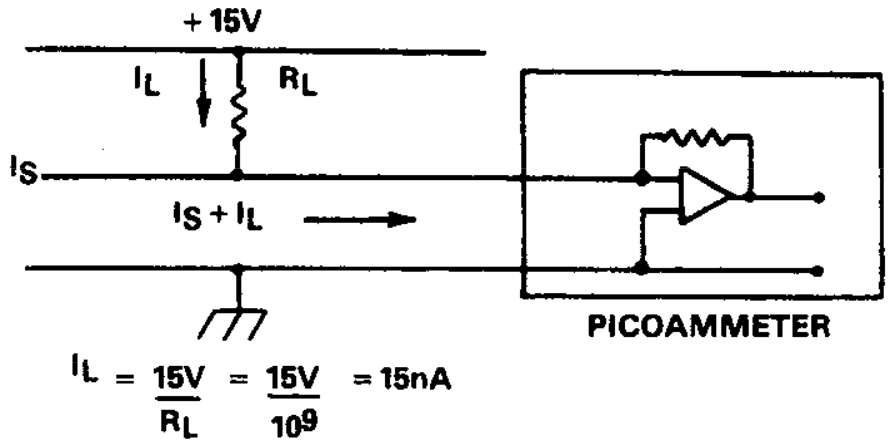
\includegraphics{figuras/instrumental/220unguarded.png}
        \caption{Sin guarda.}
        %\label{fig:posicionno}
    \end{subfigure}
    \begin{subfigure}[b]{\textwidth}
    \centering
        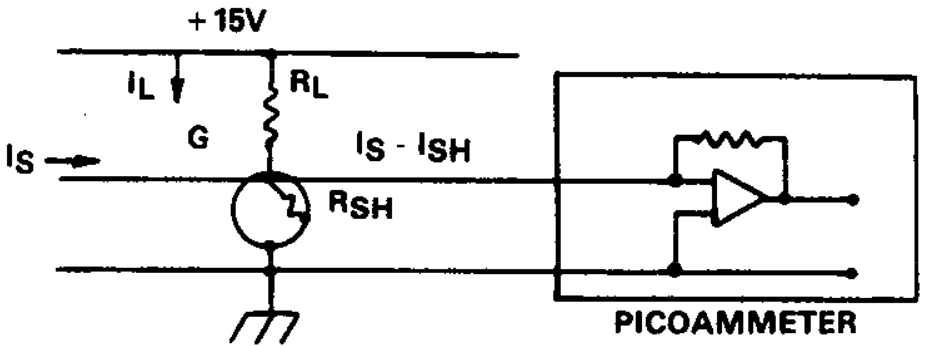
\includegraphics{figuras/instrumental/220guarded.png}
        \caption{Con guarda.}
        %\label{fig:posicionno}
    \end{subfigure}
        \caption{Efecto de las pérdidas al inyectar corriente.
        Rodeando la señal con una guarda, las corrientes de pérdida fluyen en
        la guarda y no afectan la medición.
    Reproducido de~\cite{keithley_instruments_inc._keithley_1984}.}
    \label{fig:220guard}
\end{figure}
\subsection{Módulo de adquisición de datos Keithley KUSB-3108}
El KUSB-3108 es un módulo con múltiples entradas y salidas 
analógicas y digitales controladas por una PC.
Conectando estas entradas y salidas a circuitería auxiliar,
puede reemplazar a los instrumentos anteriores para mediciones en el campo
(por ejemplo en un centro de irradiación externo).

El banco de medición del FG usa una entrada analógica del KUSB
conectada a un conversor I-V 
para medir la corriente de Drain del transistor lector.

El banco del APS usa una salida analógica 
para controlar la fuente de corriente que alimenta un LED.
Una salida digital controla la entrada de Reset de los APS,
y dos entradas analógicas miden la tensión de salida de cada sensor.
